\documentclass{article}

\usepackage{inputenc}
\usepackage{csquotes}
\usepackage[a4paper, total={6in, 10in}]{geometry}
\usepackage{hyperref}
\usepackage{amsmath,amssymb}
\usepackage{graphicx}
\usepackage{indentfirst}
\usepackage{caption}
\usepackage{subcaption}

\usepackage[backend = biber,
		   style = authoryear,
		   maxnames = 5,
		   maxcitenames = 2,
		   doi = false,
		   eprint = false]{biblatex}

\addbibresource{biblio.bib}

\title{The effect of minimum wage on rents and amenities}
\author{\textit{Gabriele Borg} \and
    \textit{Diego Gentile Passaro} \\	\small Brown University
    \and \textit{Santiago Hermo}}

\begin{document}

	\maketitle
	
\section{Introduction}

In recent years, many US jurisdictions have implemented a minimum wage (hereafter MW) above the federal minimum of \$7.25.\footnote{As of January 2020, there were 29 states that set a minimum wage higher than the federal minimum, 52 counties that set a higher minimum wage than the state, and 15 cities that set a higher minimum wage than the county.} Despite the fact that the debate on recent MW policies has been very prominent both at the local and national level, ever since \textcite{card2000minimum} most research effort has been allocated to understand the effects of MW on employment \parencite{neumark2006minimum,dube2010minimum,dube2016minimum}. This is not surprising, as employment effects are of first order importance to understand the welfare implications of MW changes. However, as MW changes are \textit{place-based} by definition, it is also natural to expect that these changes are going to affect the welfare of households through markets other than labor. By far, the most prominent candidate is the housing market. Surprisingly, there is very little research estimating the effects of MW on rents\footnote{To our knowledge the only papers aiming at answering this question are \textcite{yamagishi2019minimum} and \textcite{tidemann2018mw}. Surprisingly, they both found opposing results despite using the same year-county data. \textcite{yamagishi2019minimum} find a small positive effect, while \textcite{tidemann2018mw} finds a small negative effect. \textcite{yamagishi2019minimum} attributes this difference to different model specifications, and argues that with proper standard errors clustering the results in \textcite{tidemann2018mw} are statistically insignificant. We will soon explain the differences of this paper with those.} and house values, and virtually no research estimating the effects on local amenities. 

 A canonical version of the Alonso-Muth-Mills model\footnote{See \textcite{brueckner1987structure} for a complete treatment.} with homogeneous agents predicts that wage increases should be fully capitalized by landlords, as workers end up paying higher rents in all locations. However, how big is the pass-through from a MW change to rents has not been clearly estimated. This simple example, illustrates how the welfare implications and incidence of a MW change may very well depend on what happens with rents. Furthermore, if the pass-through to rents is high, we may also expect a response of local amenities through residential sorting. As recently emphasized by \textcite{diamond2016determinants}, accounting for the welfare implications of amenities may also be important.
 
 In this paper, we use data at the zipcode-month level to assess the reduced form effects of MW changes on rents, house values, and amenities. In the future, we hope to develop a spatial equilibrium model with agents that trade-off wages and amenities heterogeneously.\footnote{We are currently working on this model.} The model we have in mind has two types of agents (high and low), and many discrete locations. We want to derive theoretical predictions on equilibrium rents and amenities when we change exogenously the wage of the low type workers in some locations and not in others. We also have in mind to extend the model to allow for different land availability in different locations, as places we expect locations with tighter land availability to have bigger rent increases than locations with more available land (and therefore with a more elastic housing supply). 

Estimating empirically the pass-through from MW to rents is not only policy relevant, but is also of theoretical interest. As shown by \textcite{agarwal2019minimum}, if landlords know that their tenants have more disposable income raising the rent will have two theoretical effects. On one hand, it increases the landlords revenue conditional on receiving the rent payment. On the other hand, it increases the probability of tenants defaulting their payment. 

Estimating that pass-through is also challenging. It requires exogenous variation on the MW, but it is plausible that the determinants of the changes in the MW are correlated with geographical and time factors that also affect the housing market directly. 
 
To overcome this challenge, we use a panel event-study methodology \parencite{abraham2018estimating,borusyak2017revisiting} at the zipcode-month level exploiting the fine timing of hundreds of MW changes across different US jurisdictions from 2010 to 2019. As the MW changes are staggered across zipodes and dates, controlling for geographic fixed effects and geography-specific time fixed effects (among other things) we will only use within zipcode variation around the relative time of the event to estimate the relevant pass-through. This yields the causal effect assuming that factors leading to MW changes are not related to unobservable factors affecting rents. Although we cannot directly, test that assumption, in practice, the usual way of assessing its plausibility is by making sure that in the event study regression of an outcome the pre-event coefficients have no trend, as that implies that leading to the event the outcome was not trending\footnote{Recent work by \textcite{roth2018pre} has developed methods to integrate pre-trend testing into the design to get correct standard error coverage.}. In addition, pooling hundreds of MW changes in an event study is more likely to be externally valid than research based on a few case studies. 

%%%% Our results are bla bla bla

Our approach has several differences with respect to the past papers. Both \textcite{tidemann2018mw} and \textcite{yamagishi2019minimum} use Fair Markets Rents data which is available at the year-county level.\footnote{\textcite{yamagishi2019minimum} also uses data at the year-prefecture level for the 47 Japanese prefectures.} An important advantage of our approach is that we use the exact timing of the MW change at the monthly level. When using variation at the year level the event period is "partially treated" which will tend to understate the magnitude of the effect. Furthermore, some jurisdictions have MW changes on many subsequent years, making it challenging to estimate the dynamics around changes that are followed by changes in the immediate year. For example, if there is a change in two subsequent years, then the estimated effect of the change in the second year may be due too the effect of the current MW change or to the past MW change or both.

A second important difference, is that we use data at the zipcode level instead of at the county.\footnote{As of 2019 there were 3142 counties and 39295 meaningful zipcodes\footnote{We exclude military and unique business zipcodes as they are irrelevant for house prices.} in the US.} To illustrate why this is important think about the following example. For simplicity suppose that in a certain county, just before a MW change, all low skill jobs are in one particular zipcode. Suppose further that low skill households prefer to live near their jobs. Now, there is a MW increase. Suppose, consistently with \textcite{card2000minimum} and \textcite{cengiz2019effect}, that employment effects are near zero. Then, one should expect demand for housing in the zipcode with the low skill jobs to increase and demand for housing in the rest of the zipcodes to go down. If we focus, on the effects of the MW increase on the county we might even find that the rents go down, when in fact the rents in the zipcodes were the low skill jobs are will increase. Indeed, \textcite{tidemann2018mw} found that a \$1 increase in the MW decreases the yearly average of the monthly rent by 1.5 percentage points\footnote{As pointed out by \textcite{tidemann2018mw}, the sign of this effect implies that the labor demand for low skilled workers is elastic. This is at odds with the results from \textcite{card2000minimum}, \textcite{cengiz2019effect}, and many others.}. If we add amenities to the example, matters become much more complicated but if we allow for high skill people to value amenities differently than low skill people (like in \textcite{diamond2016determinants}), we may also expect to see residential resorting of high skill people depending on where are the amenities located, whether the amenities respond endogenously to the high-low skill composition of the zipcode, and depending on which are the zipcodes that the low skilled workers are demanding less. This example, illustrates that as the spatial distribution of jobs and amenities varies at the very local level, when tastes are heterogeneous by skill (or some other dimension) focusing on a large geographic area may be misleading. A second advantage of having a more detailed geography is that we can use the census to compute the level of employment and the distribution of income in each zipcode, and check if we observe stronger effects on rents in places where there are more MW earners or in places where there is more low skilled employment. 

A third important difference of our approach is that by exploiting data at the zipcode-month level we can go well beyond two-way county-year fixed effects. Our baseline specification has zipcode fixed effects, state-specific year-month fixed effects, and county-specific calendar-month fixed effects that allow for very flexible seasonal patterns. This in turn has two important advantages. First, it makes our estimates much more precise than the previous ones. Second, and most important, it makes substantially more plausible the needed identification assumptions. Given that the identifying variation comes from within zipcodes, the determinants of these MW changes are unlikely to be related to the zipcode, and therefore, are less likely to be correlated to the unobservable determinants of rents in that zipcode.

A fourth important difference with the past work, is that to the best of our knowledge, this is the first study that estimates the effect of MW changes on amenities. As pointed out recently by \textcite{diamond2016determinants, almagro2019location}, taking into account non-pecuniary dimensions of the utility function can change substantively the welfare computations and the incidence of policy relevant changes. We exploit the use of high frequency GPS data to build amenity measures at the zipcode-month level and estimate the effect of MW changes on them. We hope that by incorporating amenities into the picture we can give a more comprehensive assessment of the effects of MW policies.

Another difference with the past work is that, given the spatial granularity of our data, we can use MW changes at any jurisdictional level. This is interesting because MW changes at different jurisdiction levels may have different local effects on rents. Intuitively, this is the case because, for example, out-of-state migration is in principle more costly than out-of-county migration, therefore, we expect more residential resorting within a state and across counties when a county changes their local MW wage. Our data allows us to study the heterogeneous effects of different MW changes.\footnote{In principle, our data allows us to answer whether the effects of changes at the federal, state, county, and city/town level are different.} 

Beyond, the contribution to the very recent literature on the effects of MW changes on rents, we contribute to several strands of the literature. First, we contribute to the literature studying the effects of minimum wages on the welfare of low skill households. However, instead of focusing on wages and employment\parencite{dinardo1995labor, autor2016contribution, card2000minimum, neumark2006minimum, jardim2017minimum}, we contribute to this strand by taking into account the effects on the housing market.

Second, our work relates to the literature that studies the location decision of agents either based on income \parencite{roback1982wages, kennan2011effect, desmet2013urban, perez2018city} or based on spatial rent and amenity differentials \parencite{diamond2016determinants,almagro2019location,couture2019income, bayer2004equilibrium}. We hope to contribute by adapting this framework to the case of the MW changes, so that we can rationalize through residential location sorting part of the observed reduce form effect on rents and amenities. 

% incorporates the response of spatially differentiated amenities into place, in particular 

 \section{Data and Sample Selection Criteria}

For the entire US, we assemble a panel at the US postal service zipcode-month level from January 2010 to December 2019. This panel that comes from five distinct sources. 

First, our data contains prominent MW changes at the federal, state, county, and city level.\footnote{Note that federal level MW changes still induce meaningful variation as it is binding in some zipcodes and not in others, so that identification don't come only from time series variation. In our baseline estimates we exclude county and city level changes because they might have different effects on rents and amenities. We include prominent MW changes at those levels in robustness checks, and in specifications that allow explicitly for heterogeneous effects at the different jurisdiction levels.} Most of these changes come from \textcite{vaghul2016historical} and \textcite{cengiz2019effect}, but we updated this data for the years 2017, 2018, and 2019. For each zipcode we only use MW changes that are binding, and that are prominent. We define a MW change as prominent when it is of at least \$0.5 following closely \textcite{cengiz2019effect}\footnote{We conduct for changes of at least \$0.25 and \$0.75.}. We only use MW event changes that have at least 6 months of data after the month of the event.\footnote{For example, if an event happened in July 2019 we would exclude it from our sample of events.} Finally, to avoid dealing with overlapping events, our baseline specifications uses a 6 months window period around the latest MW change event that satisfies our criteria for each zipcode. In robustness checks we follow the methodology of \textcite{cengiz2019effect} to use all events and results are very similar.

Second, we use rent and house value data from properties listed in Zillow \parencite{zillow} in our sample period. To make sure that our data is representative of the time series of the housing market in the US, we compare it with the Fair Market Rents data coming from the US Department of Housing and Urban Development \parencite{hud}, and with the Case-Shiller 20-City Composite Home Price Index \parencite{case}. To ease comparison across zipcodes, we focus on rent and house prices per square foot for single family houses. For this category the Zillow data provides information on rents for 3316 unique zipcodes that correspond to \%8.43 of the zipcodes and to \%36.6 of the 2015 population. The average median household annual income for those zipcodes in 2015 was \$75209, which is \%26.6 higher than the same figure for all the US zipcodes. As for the information on house values, Zillow has data on 10875 unique zipcode that correspond to \%27.7 of the zipcodes and to \%78.9 of the 2015 population. The average median household annual income for those zipcodes in 2015 was \$69556, which is \%17 higher than the same figure for all the US zipcodes. Therefore, our zipcodes are more populous and slightly higher income than the average zipcode. 

Third, we assign to each USPS zipcode a Zip Code Tabulation Area (ZCTA) and we use the census at that level to assign to each zipcode the number of inhabitants, the number of houses, and the median income. We use this information to classify zipcodes into high or low population (or population density) and into high or low median income. In addition, given that zipcodes can cross county borders, we use the census data and geographic codes to map each zipcode to a county by assigning it to the one that has the highest share of houses from that zipcode among all counties in which the zipcode has houses. We also map to each zipcode to a metropolitan statistical area or a rural town analogously.

Fourth, to proxy for the quality of amenities at each location, we construct zipcode-month level measures from GPS location point-of-interest data by SafeGraph\parencite{safegraph}. We define several amenity measures. For our first measure, we follow closely \textcite{couture2019income} and construct an index for the quality of restaurants available at each zipcode-month. This index is defined as the average of the propensity of high-income individuals to visit a restaurant in a given zipcode controlling for their distance to the establishments. In order to classify a visitor as high-income we use the census tract location of the visitor. Our second measure is the same as the first but for the quality of the visitors of open public spaces in each zipcode-month. For our third measure, we use the point-of-interest data to count the number of restaurants, coffee shops, bars, and gyms per inhabitant of a zipcode-month. 

Finally, we collect data from the Quarterly Census of Employment and Wages at the county-quarter level. For each county-quarter, and for each 5-digit NAICS industry code, we observe the number of establishment, the number of employed people, and the average weekly wage. We merge this data into our zipcode-month panel, based on the county and quarter that they belong, and we classify counties into high or low wage areas, or into high or low employment area, and for building controls on the level of employment and economic activity. 

\section{Empirical Strategy and Identification}

As stated before, we use a panel event-study methodology exploiting the fine timing of hundreds of MW changes staggered across zipcodes and months. These high frequency data allows for simultaneous identification of relative dynamics around the event and a very rich set of fixed effects. In particular, we use location fixed effects, county-specific time fixed effects, and county-specific calendar month fixed effects (to account for flexible seasonal pattern at the local level). The specification that we are using is given by:

\begin{equation}
\begin{aligned}
    y_{jt} = \sum\limits_{k = -w}^{-2}\delta_{t + k} D_{j(t+k)} + \sum\limits_{k = 0}^{w}\delta_{t + k} D_{j(t + k)} + \alpha_{j} + \alpha_{ct} + \boldsymbol{\beta} \boldsymbol{X}_{jt} +\epsilon_{jt} 
\end{aligned}   
\end{equation}

where

\begin{itemize}
    \item $j$: zipcode
    \item $t$: time
    \item $w$: event window
    \item $c$: county.
    \item $D_{j (t + k)}$: indicator for MW change in zipcode $j$ in period $t+k$
    \item $\boldsymbol{X}_{it}$: time and spatial controls (e.g. county-specific calendar month)\footnote{If a given zipcode always experience MW changes in a particular calendar month, say January, these fixed effects will partial out that effect from the dynamics. As there are many zipcodes that experience changes at different calendar months, those effects are identified jointly to the dynamic treatment effects. }
\end{itemize}

The main identifying assumption is that $E \left( \epsilon_{jt} D_{j(t+k)} | \alpha_j, \alpha_{ct}, \boldsymbol{\beta} \boldsymbol{X}_{jt}\right)  = 0  \ \ \ \forall k\in[-w, w]$. Intuitively, this means that unobservable determinants of the outcome are mean independent from the relative timing of the MW event conditional on the set of fixed effects and controls. In our context, as we use within zipcode variation this assumption seems much more plausible than the assumptions needed when using within county variation and a much less flexible set of fixed effects. Conditional on county-specific time fixed effects and county-specific calendar months\footnote{Note that these fixed effects are a very high dimensional object.}, the unobserved within zipcode variation is unlikely to be correlated with the determinants of the timing of the MW change, as these latter are plausibly not determined at the zipcode level. One important reason for this is that MW changes are usually enacted through federal or state law, or through local ordinances that are subject to higher level court blocks and revisions, and that may follow from ballot initiative. Therefore, the timing of the enactment of a MW change in a given zipcode could be thought as random. Furthermore, federal and state changes are, for the overwhelming majority of zipcodes, unarguably determined far from the zipcode political influence. 

We will discuss the no pre-trends assumption in the next section.

\section{Preliminary Results}

\subsection{Rents}

Figure \ref{fig:fig1}\footnote{Code producing the analysis in this section can be found in \url{https://github.com/diegogentilepassaro/min_wage_rent}} plots the relative event coefficients of a regression like (1) for single family rents per square foot for MW events of at least \$0.5. 

\begin{figure}[h!]
    \centering
    \scalebox{0.45}{
    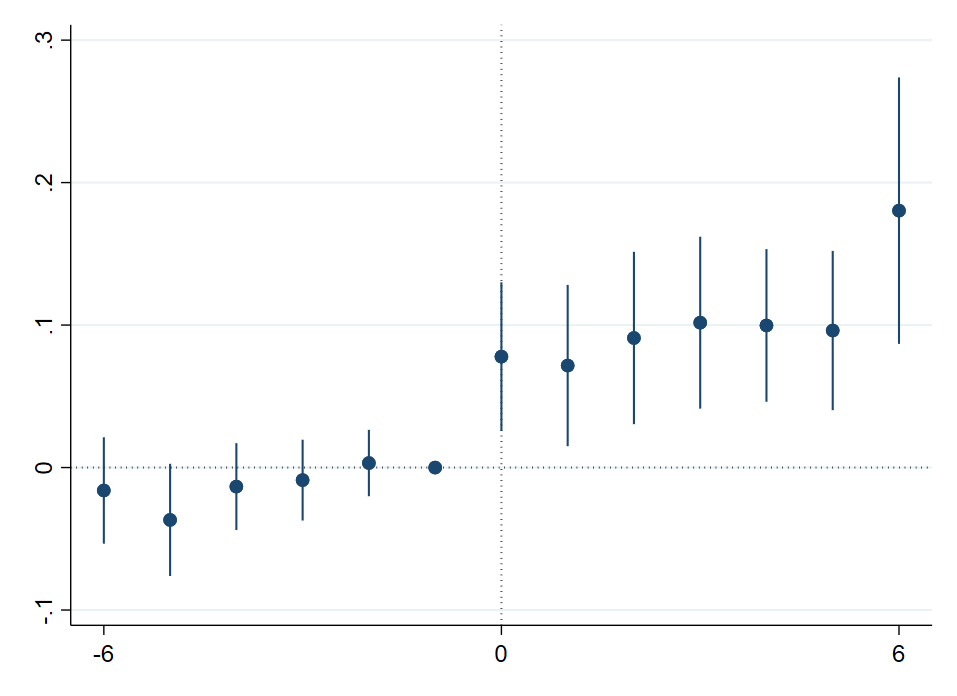
\includegraphics{../analysis/event_study/output/last_rentpsqft_sfcc_w6.png}
    }
    \caption{Baseline specification. Effects of a MW change of at least \$0.5 on single family rent per square foot (in dollars). Standard errors are clustered at the zipcode level.}
    \label{fig:fig1}
\end{figure}

The average increase of the MW change in this specification is of \$0.8. For a family of 2 minimum wagers that work 40 hours a week, given that the average month has 4.35 weeks, this change represents an increase on the family income of \$278.4. The on-impact effect on rents per square foot is of around ten cents and grows slightly in the months following the event. Assuming this representative single family consumes 1500 square feet of housing, the implied increase in monthly rent is of about \$150, which implies an on-impact pass-through from the MW change to rents of 53.9\%. If assuming that the treatment effect is given by averaging the 7 post event coefficient, then the implies pass-through is of about 64.4\%.

First note that, taken at face value this number seems slightly high given that the  median US rent requires 28.4\% of the median incomes \parencite{bi}. However, a household with 2 full time minimum wagers making, for example, the federal minimum wage of \$7.25 will have an annual income of \$30276, only slightly above half of the median US household income of \$59430 in 2015, which suggests that the estimated pass-through is plausible. 

Second, we check the robustness of this result by change the prominence of the MW changes. We use MW changes that comply to our sample criterion (explained in section 2) and are of at least \$0.25 and of at least \$0.75 instead of \$0.5. For each of the event definitions we bootstrap, clustering at the zipcode level, the whole computation of the pass-through (assuming that the relevant per square foot effect is the average of the post event coefficients). The results are presented in Table \ref{tab:table1}, where the middle column corresponds to Figure \ref{fig:fig1}. Note that we compute the implied pass-through for 3 different housing size assumptions: 1000, 1500, and 2000 square feet. We believe that those 3 values cover the range of plausible values for the average rental of a single family with 2 MW earners. Finally, note that as in any event-study, we are using only the zipcodes that have at least one MW change in our period. To gain precision, and for further robustness we are planning to use a specification that allows us to also use zipcodes that never have a MW change. Intuitively, this will help us estimate the fixed effects more precisely. 

\begin{table}[h!]
    \centering
    \resizebox{\textwidth}{!}{
    {
\def\sym#1{\ifmmode^{#1}\else\(^{#1}\)\fi}
\begin{tabular}{l*{3}{c}}
\hline\hline
            &\multicolumn{1}{c}{(1)}        &\multicolumn{1}{c}{(2)}        &\multicolumn{1}{c}{(3)}        \\
            &\multicolumn{1}{c}{MW changes of at least \$0.25}&\multicolumn{1}{c}{MW changes of at least \$0.5}&\multicolumn{1}{c}{MW changes of at least \$0.75}\\
\hline
Rent increase per square feet&                0.0139         &                0.0730\sym{*}  &                0.0687\sym{***}\\
            &     [-0.00716,0.0350]         &        [0.0136,0.132]         &        [0.0313,0.106]         \\
[1em]
Total rent increase (assuming 1000 square feet)&                 13.93         &                 72.97\sym{*}  &                 68.73\sym{***}\\
            &        [-7.161,35.03]         &         [13.57,132.4]         &         [31.34,106.1]         \\
[1em]
Total rent increase (assuming 1500 square feet)&                 20.90         &                 109.5\sym{*}  &                 103.1\sym{***}\\
            &        [-10.74,52.54]         &         [20.35,198.6]         &         [47.01,159.2]         \\
[1em]
Total rent increase (assuming 2000 square feet)&                 27.86         &                 145.9\sym{*}  &                 137.5\sym{***}\\
            &        [-14.32,70.05]         &         [27.13,264.8]         &         [62.69,212.2]         \\
[1em]
Increase in income of a household with 2 full time minimum wages&                 208.8\sym{***}&                 274.9\sym{***}&                 424.6\sym{***}\\
            &         [199.8,217.8]         &         [266.3,283.5]         &         [406.6,442.5]         \\
[1em]
Implied passthrough from MW to rents (assuming 1000 square feet)&                0.0667         &                 0.265\sym{*}  &                 0.162\sym{***}\\
            &       [-0.0352,0.169]         &        [0.0500,0.481]         &        [0.0740,0.250]         \\
[1em]
Implied passthrough from MW to rents (assuming 1500 square feet)&                 0.100         &                 0.398\sym{*}  &                 0.243\sym{***}\\
            &       [-0.0528,0.253]         &        [0.0751,0.721]         &         [0.111,0.375]         \\
[1em]
Implied passthrough from MW to rents (assuming 2000 square feet)&                 0.133         &                 0.531\sym{*}  &                 0.324\sym{***}\\
            &       [-0.0704,0.337]         &         [0.100,0.962]         &         [0.148,0.499]         \\
\hline
Minimum MW change&                               &                               &                               \\
Average MW change&                    .6         &                   .79         &                  1.22         \\
Maximum MW change&                               &                               &                               \\
Number of zipcode-months&                 59899         &                 36535         &                 30893         \\
Number of Zipcodes&                   572         &                   353         &                   299         \\
Number of bootstrap repetitions&                   181         &                   178         &                   176         \\
\hline\hline
\end{tabular}
}

    }
     \vspace{1ex}
    {\raggedright Square brackets display the 95\% bootstrapped confidence intervals. Income computations are done assuming 2 MW earners.\par}
    \caption{Bootstrapping the main objects of interest}
    \label{tab:table1}
\end{table}

Next, we show the importance of allowing for flexible year-month fixed effects that are specific to the county. Remember that is was not feasible when the unit of observation is the county. If we just include two-way fixed effects, which in our case corresponds to zipcode and year-month, all variation across time and zipcodes will end up being used estimating the relative event coefficients. But if, for example, different states or counties or MSAs have different time trends in rent prices, as it is probably the case, then the model will be misspecified. In particular, as within zipcode variation is not "de-trended", the relative event coefficients will be much harder to estimate as they will be cofounded by the trend. Figure \ref{fig:fig2} presents an event study plot analogous to Figure \ref{fig:fig1} but using a simple two-way fixed effect specification. 

\begin{figure}[h!]
    \centering
    \scalebox{0.45}{
    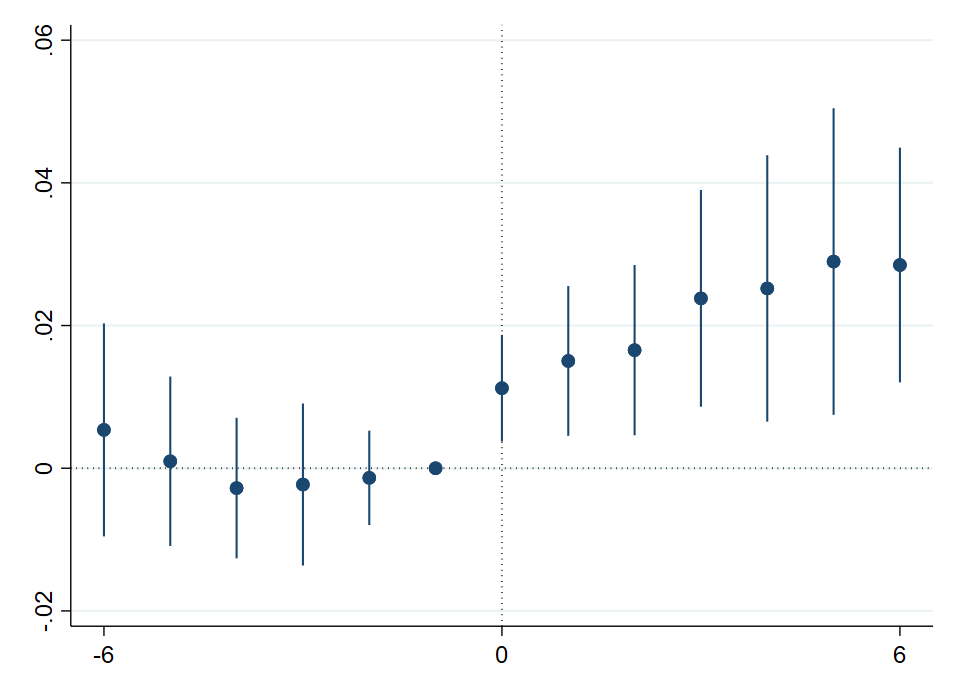
\includegraphics{../analysis/event_study/output/two_way_last_medrentpricepsqft_sfcc6.png}
    }
    \caption{Two-way fixed effects specification. Effects of a MW change of at least \$0.5 on single family rent per square foot (in dollars). Standard errors are clustered at the zipcode level.}
    \label{fig:fig2}
\end{figure}

In fact, we see that estimation of the relative coefficients is much noisier and lower in magnitude. The within variation R-squared (the percentage of the within variation in the data explained by the model) is of 0.0066. When allowing for county-specific time fixed effects and county-specific calendar months (to allow for flexible seasonality patterns) that are infeasible under the specifications in the previous literature we get \ref{fig:fig1} and a within variation R-squared of 0.0779, so that we are able to explain 12 times more within zipcode variation. These results suggest that county-specific year-month and seasonal month variation are important determinants of monthly rent at the local level above and beyond two way fixed effects.

The last result of this subsection shows what happens if we aggregate our zipcode-month data at the county-quarter level\footnote{In order to use the data in the same unit as \textcite{tidemann2018mw,yamagishi2019minimum} we should have aggregated at the county-year. However, that involves dealing with overlap in the events for each county as we have many MW changes on subsequent years. Therefore, we aggregated the data at the county-quarter under the thought that we can only do better than at the county-year. }. Figure \ref{fig:fig3} plots the relative event coefficients for a two-way fixed effect specification at the county-quarter, for a window of 2 quarters around MW changes of at least \$0.5. Similar to \textcite{tidemann2018mw} results are very imprecise and point estimates are, if anything, negative. 

\begin{figure}[h!]
    \centering
    \scalebox{0.45}{
    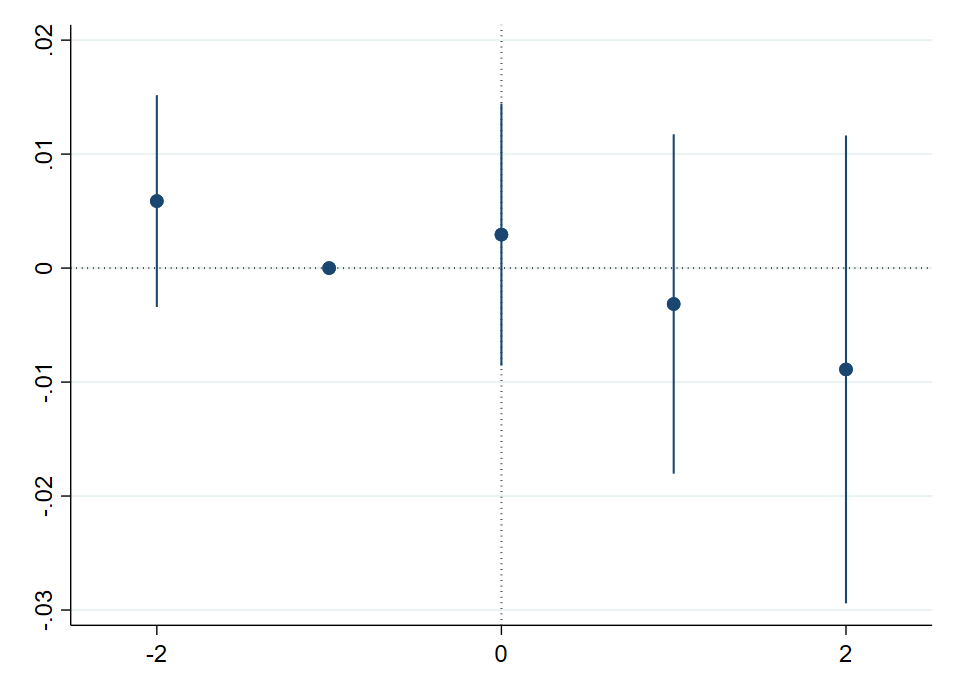
\includegraphics{../analysis/event_study_county_quarter/output/last_rentpsqft_sfcc_w2.png}
    }
    \caption{Two-way fixed effects county-quarter specification. Effects of a MW change of at least \$0.5 on single family rent per square foot (in dollars). Standard errors are clustered at the zipcode level.}
    \label{fig:fig3}
\end{figure}

\subsection{House Prices}

Figure \ref{fig:fig1} plots the relative event coefficients of a regression like (1) for single family house values per square foot for MW events of at least \$0.5. 

\begin{figure}[h!]
    \centering
    \scalebox{0.45}{
    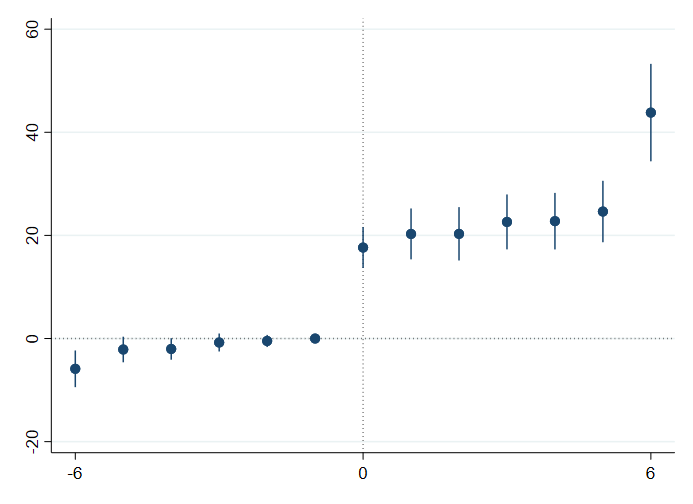
\includegraphics{../analysis/event_study/output/last_listingpsqft_sfcc_w6.png}
    }
    \caption{Baseline specification. Effects of a MW change of at least \$0.5 on single family house prices per square foot (in dollars). Standard errors are clustered at the zipcode level.}
    \label{fig:fig4}
\end{figure}

The effect on house values per square foot is of around \$12.5. If we take a purely financial perspective that house values are the present discounted value of perpetuity, we can compute the implied interest rate from the increase in the per square foot present discounted value of \$12.5 (heareafter PDV) and the increase in a monthly cash flows of around \$0.10 cents from section 4.1 (hereafter CF).

\begin{equation}
    PDV = \frac{CF}{r} \to r = \frac{CF}{PDV}
\end{equation}

For our case, the implied monthly interest rate is of 0.008 which implies an annual interest rate of around 10\%. This seems like a very high interest rate, although is not totally implausible. It could potentially be rationalized if agents also expect capital gains on the house, or if agents are also capitalizing future MW changes (as they might expect that a MW change in a given location means that more MW changes may come in the future). Further analyzing these results is work for the future. 

\subsection{Amenities}

For the future. 

\section{Model}

For the future.

\section{Conclusions}

For the future.

\section{New stuff}

\begin{table}[h!]
    \centering
    \resizebox{\textwidth}{!}{
    {
\def\sym#1{\ifmmode^{#1}\else\(^{#1}\)\fi}
\begin{tabular}{l*{3}{c}}
\hline\hline
          &\multicolumn{1}{c}{(1)}&\multicolumn{1}{c}{(2)}&\multicolumn{1}{c}{(3)}\\
          &\multicolumn{1}{c}{D.ln\_med\_rent\_psqft}&\multicolumn{1}{c}{D.ln\_med\_rent\_psqft}&\multicolumn{1}{c}{D.ln\_med\_rent\_psqft}\\
\hline
D.ln\_mw   &   0.0257\sym{*}  &   0.0253\sym{**} &   0.0250\sym{**} \\
          & (0.0128)         & (0.0121)         & (0.0117)         \\
\hline
Zipcode-specifc linear trend&       No         &      Yes         &      Yes         \\
Zipcode-specific linear and square trend&       No         &       No         &      Yes         \\
R-squared &                  &                  &                  \\
Observations&    0.022         &    0.023         &    0.026         \\
N         &   113363         &   113363         &   113363         \\
\hline\hline
\end{tabular}
}

    }
     \vspace{1ex}
    {\raggedright Standard errors in parenthesis are clustered at the state level.\par}
    \caption{First-differences specification.}
    \label{tab:table1}
\end{table}

\begin{table}[h!]
    \centering
    \resizebox{\textwidth}{!}{
    {
\def\sym#1{\ifmmode^{#1}\else\(^{#1}\)\fi}
\begin{tabular}{l*{5}{c}}
\hline\hline
          &\multicolumn{1}{c}{(1)}         &\multicolumn{1}{c}{(2)}         &\multicolumn{1}{c}{(3)}         &\multicolumn{1}{c}{(4)}         &\multicolumn{1}{c}{(5)}         \\
\hline
$\Delta \ln \underline{w}_{ic,t-5}$&  -0.0148         &  -0.0144         &  -0.0144         &  -0.0146         &  -0.0144         \\
          & (0.0090)         & (0.0089)         & (0.0089)         & (0.0090)         & (0.0089)         \\
[1em]
$\Delta \ln \underline{w}_{ic,t-4}$&  -0.0024         &  -0.0019         &  -0.0020         &  -0.0022         &  -0.0019         \\
          & (0.0116)         & (0.0116)         & (0.0115)         & (0.0116)         & (0.0115)         \\
[1em]
$\Delta \ln \underline{w}_{ic,t-3}$&   0.0011         &   0.0005         &   0.0007         &   0.0004         &  -0.0002         \\
          & (0.0092)         & (0.0094)         & (0.0092)         & (0.0091)         & (0.0092)         \\
[1em]
$\Delta \ln \underline{w}_{ic,t-2}$&   0.0060         &   0.0063         &   0.0062         &   0.0060         &   0.0064         \\
          & (0.0116)         & (0.0118)         & (0.0116)         & (0.0115)         & (0.0117)         \\
[1em]
$\Delta \ln \underline{w}_{ic,t-1}$&  -0.0002         &  -0.0004         &  -0.0005         &   0.0000         &  -0.0005         \\
          & (0.0123)         & (0.0123)         & (0.0124)         & (0.0122)         & (0.0123)         \\
[1em]
$\Delta \ln \underline{w}_{ic,t}$&   0.0271\sym{**} &   0.0257\sym{**} &   0.0259\sym{**} &   0.0269\sym{**} &   0.0259\sym{**} \\
          & (0.0126)         & (0.0123)         & (0.0124)         & (0.0126)         & (0.0124)         \\
[1em]
$\Delta \ln \underline{w}_{ic,t+1}$&   0.0136\sym{*}  &   0.0146\sym{**} &   0.0142\sym{*}  &   0.0135\sym{*}  &   0.0146\sym{*}  \\
          & (0.0072)         & (0.0072)         & (0.0072)         & (0.0072)         & (0.0072)         \\
[1em]
$\Delta \ln \underline{w}_{ic,t+2}$&  -0.0070         &  -0.0066         &  -0.0064         &  -0.0068         &  -0.0064         \\
          & (0.0133)         & (0.0133)         & (0.0132)         & (0.0133)         & (0.0132)         \\
[1em]
$\Delta \ln \underline{w}_{ic,t+3}$&   0.0036         &   0.0045         &   0.0047         &   0.0031         &   0.0040         \\
          & (0.0081)         & (0.0078)         & (0.0078)         & (0.0079)         & (0.0077)         \\
[1em]
$\Delta \ln \underline{w}_{ic,t+4}$&   0.0108         &   0.0093         &   0.0104         &   0.0107         &   0.0096         \\
          & (0.0069)         & (0.0066)         & (0.0064)         & (0.0069)         & (0.0065)         \\
[1em]
$\Delta \ln \underline{w}_{ic,t+5}$&   0.0086         &   0.0095         &   0.0099         &   0.0088         &   0.0099         \\
          & (0.0069)         & (0.0065)         & (0.0065)         & (0.0067)         & (0.0065)         \\
\hline
\vspace{-2mm}&                  &                  &                  &                  &                  \\
Cumulative effect&    0.057         &0.057\sym{*}         &0.059\sym{*}         &    0.056         &0.058\sym{*}         \\
          &  (0.035)         &  (0.034)         &  (0.034)         &  (0.034)         &  (0.034)         \\
\hline    &                  &                  &                  &                  &                  \\
P-value no pretrends&    0.568         &    0.612         &    0.599         &    0.594         &    0.629         \\
Wage controls&       No         &      Yes         &       No         &       No         &      Yes         \\
Employment controls&       No         &       No         &      Yes         &       No         &      Yes         \\
Establishment-count controls&       No         &       No         &       No         &      Yes         &      Yes         \\
R-squared &    0.022         &    0.022         &    0.022         &    0.022         &    0.022         \\
Observations&  106,446         &  105,463         &  105,463         &  106,160         &  105,463         \\
\hline\hline
\end{tabular}
}

    }
     \vspace{1ex}
    {\raggedright Standard errors in parenthesis are clustered at the state level.\par}
    \caption{First-differences specification.}
    \label{tab:table1}
\end{table}

\begin{table}[h!]
    \centering
    \resizebox{\textwidth}{!}{
    {
\def\sym#1{\ifmmode^{#1}\else\(^{#1}\)\fi}
\begin{tabular}{l*{3}{c}}
\hline\hline
          &\multicolumn{1}{c}{(1)}&\multicolumn{1}{c}{(2)}&\multicolumn{1}{c}{(3)}\\
          &\multicolumn{1}{c}{D.ln\_med\_rent\_psqft\_sfcc}&\multicolumn{1}{c}{D.ln\_med\_rent\_psqft\_sfcc}&\multicolumn{1}{c}{D.ln\_med\_rent\_psqft\_sfcc}\\
\hline
Sum of MW effects&   0.0567         &   0.0520         &   0.0474         \\
          & (0.0346)         & (0.0335)         & (0.0301)         \\
\hline
Zipcode-specifc linear trend&       No         &      Yes         &      Yes         \\
Zipcode-specific quadratic trend&       No         &       No         &      Yes         \\
Observations&                  &                  &                  \\
N         &  106,446         &  106,446         &  106,446         \\
\hline\hline
\end{tabular}
}

    }
     \vspace{1ex}
    {\raggedright Standard errors in parenthesis are clustered at the state level.\par}
    \caption{First-differences specification.}
    \label{tab:table1}
\end{table}

\nocite{*}
\printbibliography


% \begin{figure}[h!]
% \centering
% \begin{subfigure}{.5\textwidth}
%   \centering
%   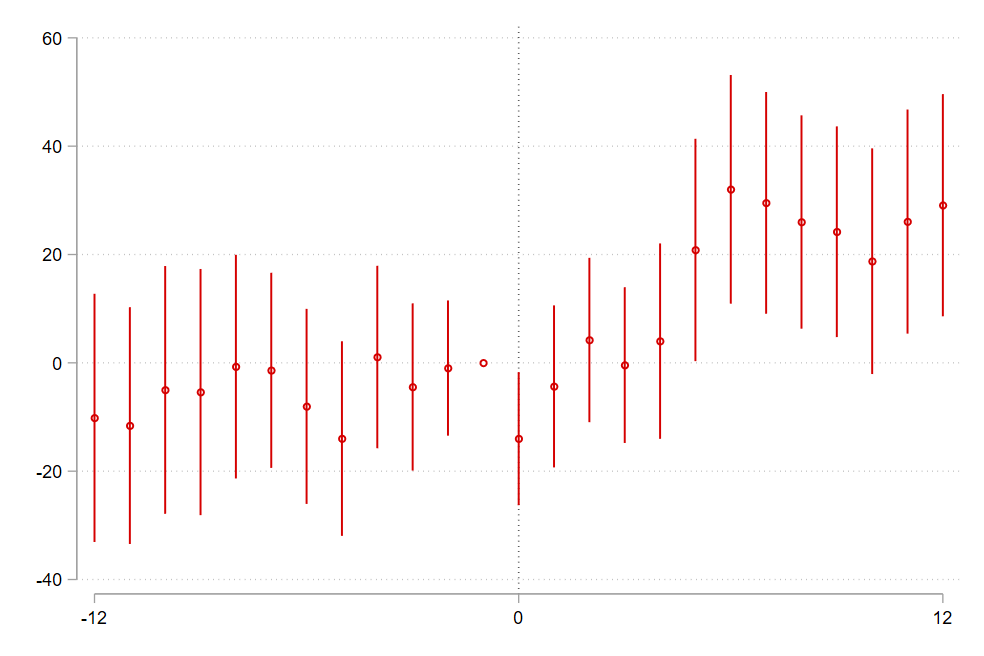
\includegraphics[width=.8\linewidth]{rent2br_median_rel_months_min_event12.png}
%   \caption{12 month window}
%   \label{fig:sub1}
% \end{subfigure}%
% \begin{subfigure}{.5\textwidth}
%   \centering
%   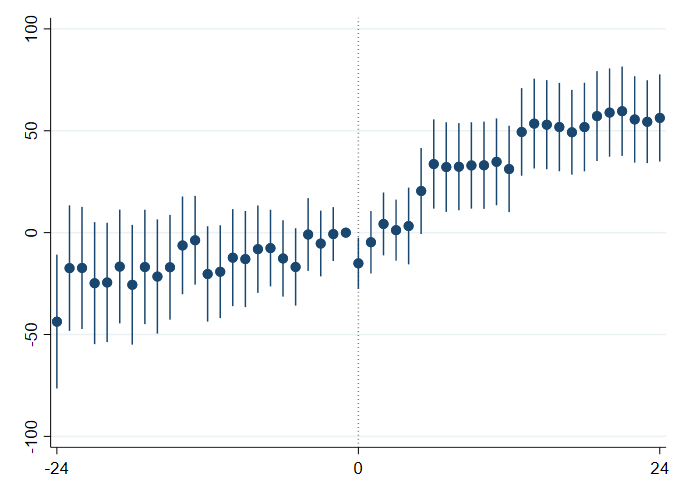
\includegraphics[width=.8\linewidth]{rent2br_median_rel_months_min_event24.png}
%   \caption{24 month window}
%   \label{fig:sub2}
% \end{subfigure}
% \caption{Median rent for a 2 bedroom}
% \label{fig:test}
% \end{figure}

% \begin{figure}[h!]
% \centering
% \begin{subfigure}{.5\textwidth}
%   \centering
%   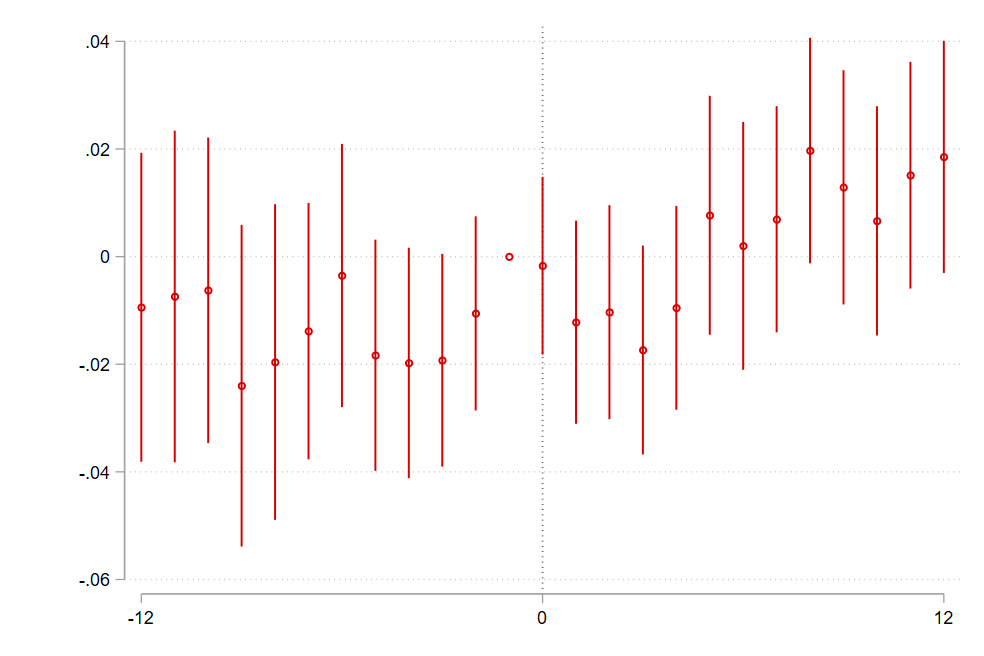
\includegraphics[width=.8\linewidth]{rent2br_psqft_median_rel_months_min_event12.png}
%   \caption{12 month window}
%   \label{fig:sub1}
% \end{subfigure}%
% \begin{subfigure}{.5\textwidth}
%   \centering
%   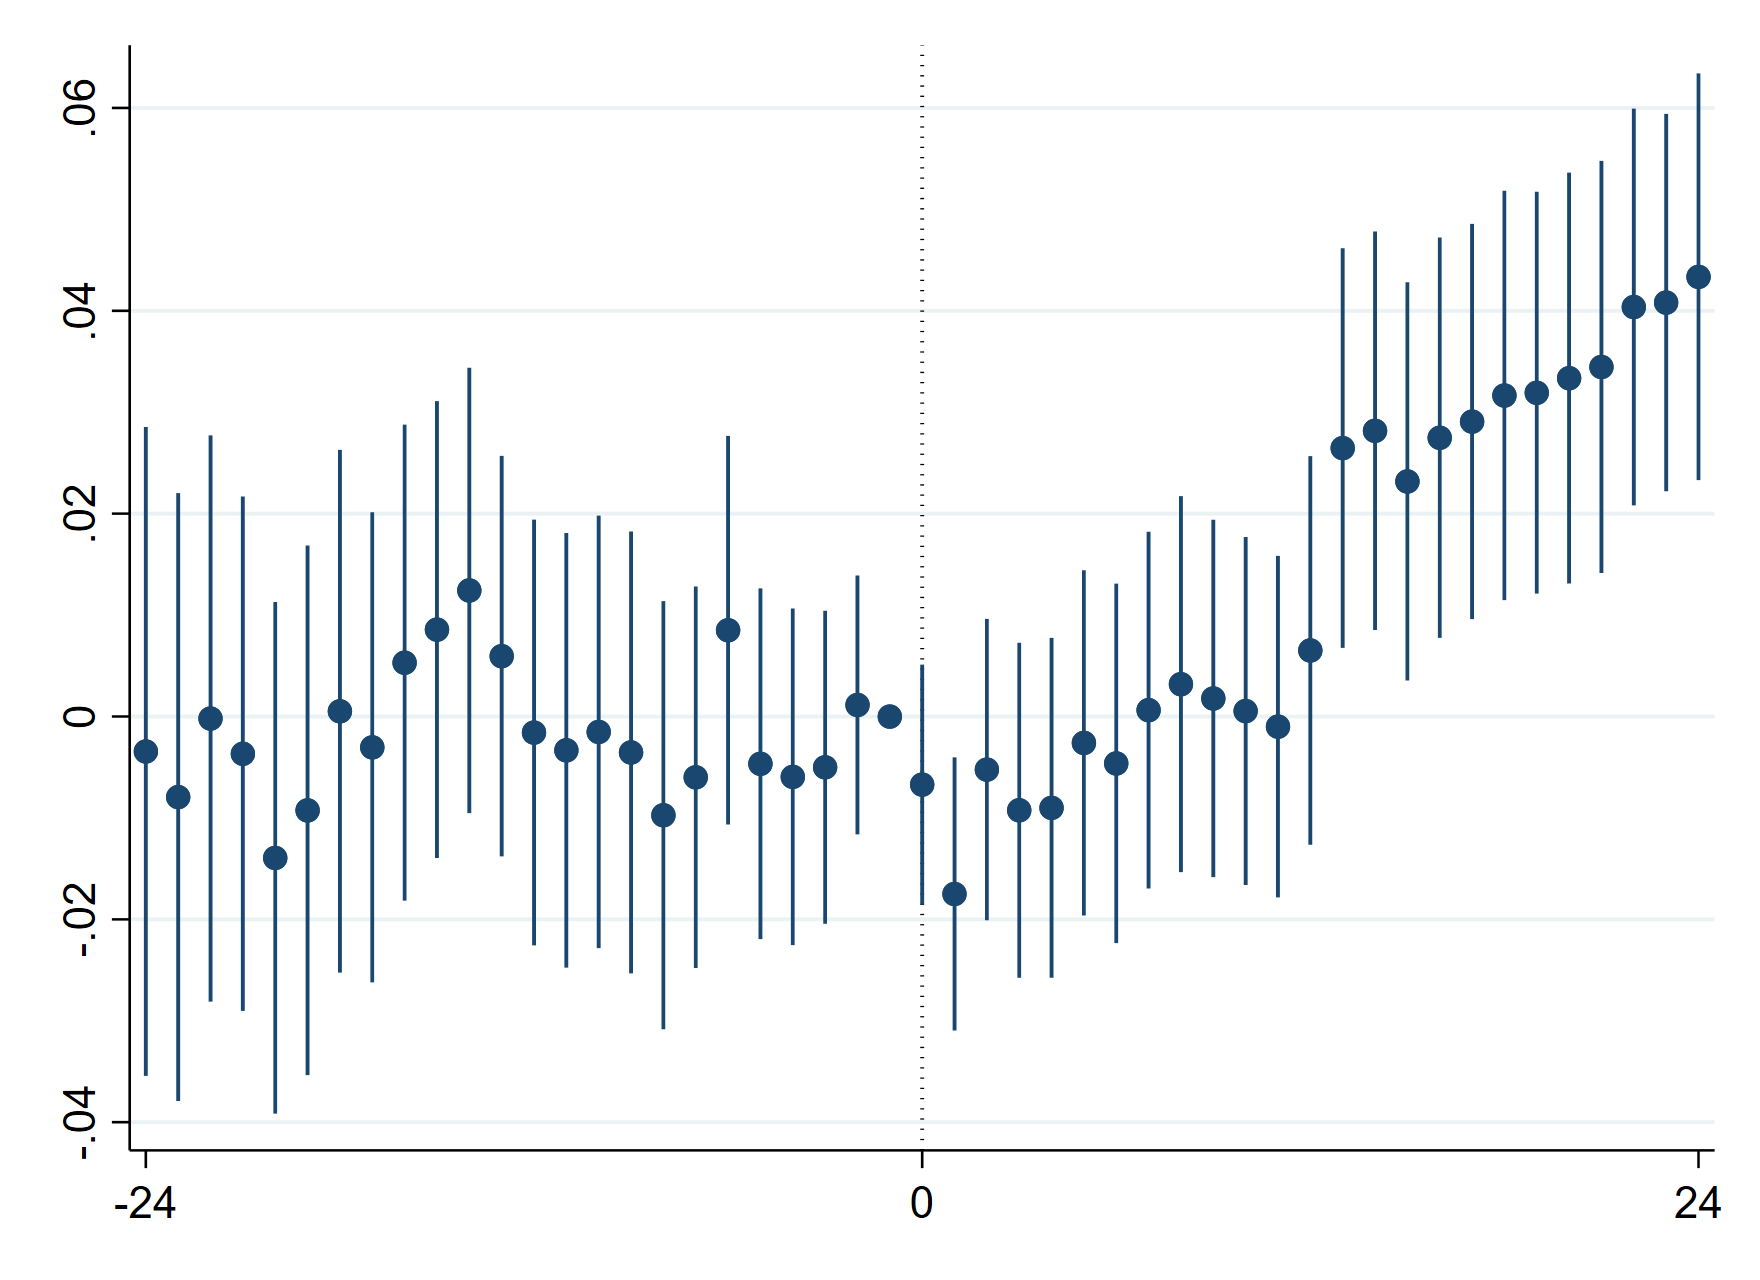
\includegraphics[width=.8\linewidth]{rent2br_psqft_median_rel_months_min_event24.png}
%   \caption{24 month window}
%   \label{fig:sub2}
% \end{subfigure}
% \caption{Median rent per square foot for a 2 bedroom}
% \label{fig:test}
% \end{figure}

\end{document}